% -*- coding: utf-8 -*-
% !TEX program = xelatex
\documentclass[14pt,notheorems]{beamer}
\usetheme[style=beta]{epyt} % alpha, beta, delta, gamma, zeta
\usepackage[UTF8,noindent]{ctex}
\usepackage{url}
\usepackage{graphicx}
\usepackage{xcolor}
\setcounter{section}{2}
\usepackage{listings}
\lstset{
  basicstyle=\ttfamily,xleftmargin=0em,
  commentstyle=\color{teal},keywordstyle=\color{acolor4},
  language=[LaTeX]{TeX},morekeywords={usetheme,epytsetup}
}

\newcommand{\mylead}[1]{\textcolor{acolor1}{#1}}
\newcommand{\mybold}[1]{\textcolor{acolor2}{#1}}
\newcommand{\mywarn}[1]{\textcolor{acolor3}{#1}}

%\newtheorem{theorem}{定理}
%\newtheorem{definition}[theorem]{定义}
%\newtheorem{example}[theorem]{例子}
%\renewcommand{\proofname}{证明}
%\newtheorem*{theorem*}{定理}
%\newtheorem*{definition*}{定义}
%\newtheorem*{example*}{例子}
\begin{document}
\title{\TeX studio 简介与安装使用}
\author{枫随风落}
\date{\today}
\begin{frame}[plain]\transboxout
\titlepage
\end{frame}

\begin{frame}\transboxin
\begin{itemize}
	\frametitle{主流\TeX{}编辑器介绍}%主标题
	%\framesubtitle{副标题演示}%副标题
	\item WinEdt 收费\LaTeX{}编辑器,功能强大
	\item TeXworks MikTeX 和TexLive 自带编辑器
	\item TeXStudio 免费开源编辑器,某些功能可以媲美Winedt
	\item TeXmaker 功能丰富
	\item Vim,Notepad++,Emacs,Kile 需要安装相应插件
\end{itemize}
\end{frame}

%\begin{frame}{1.几种编辑器的介绍}
%\vspace{-1.5cm}
%%\mylead{} 几款主要的编辑器:\pause
%\begin{itemize}%[<+->]
%\item WinEdt:这是CTeX自带的一款,功能比较齐全,也是我的入门编辑器。(\TeX friend)
%\item TeXworks:这个是TeXlive自带的一款,轻量级的。
%\item 其他:Sublime Text 、ShareLaTeX(在线)、Emacs 、\mylead{\TeX studio} 
%\end{itemize}
%\end{frame}

\begin{frame}{2.\TeX studio特点与下载地址}
%	\mylead{Epyt} 主题已经包含在主要的 TeX 发行版中。
\vspace{-1.5cm}
优点:
	\begin{itemize}
		\item TexStudio 具有TexWorks 一切优点,功能更加齐全%,例如拼写检查,代码自动补全,折叠,查找支持表达式,支持正向与反向搜索等
		\item 跨平台、开放源代码
		\item 用户界面美观,可定制性极强
		\item 具有版本控制功能,比如SVN
	\end{itemize}
缺点:
\begin{itemize}
	\item 某些功能不如WinEdt,使用Qt 5 开发,有一些小bug
\end{itemize}
下载地址:
	\url{http://www.texstudio.org/}
	
\end{frame}

\section{\TeX studio下载安装过程演示}
\begin{frame}
	\begin{figure}
		\centering
		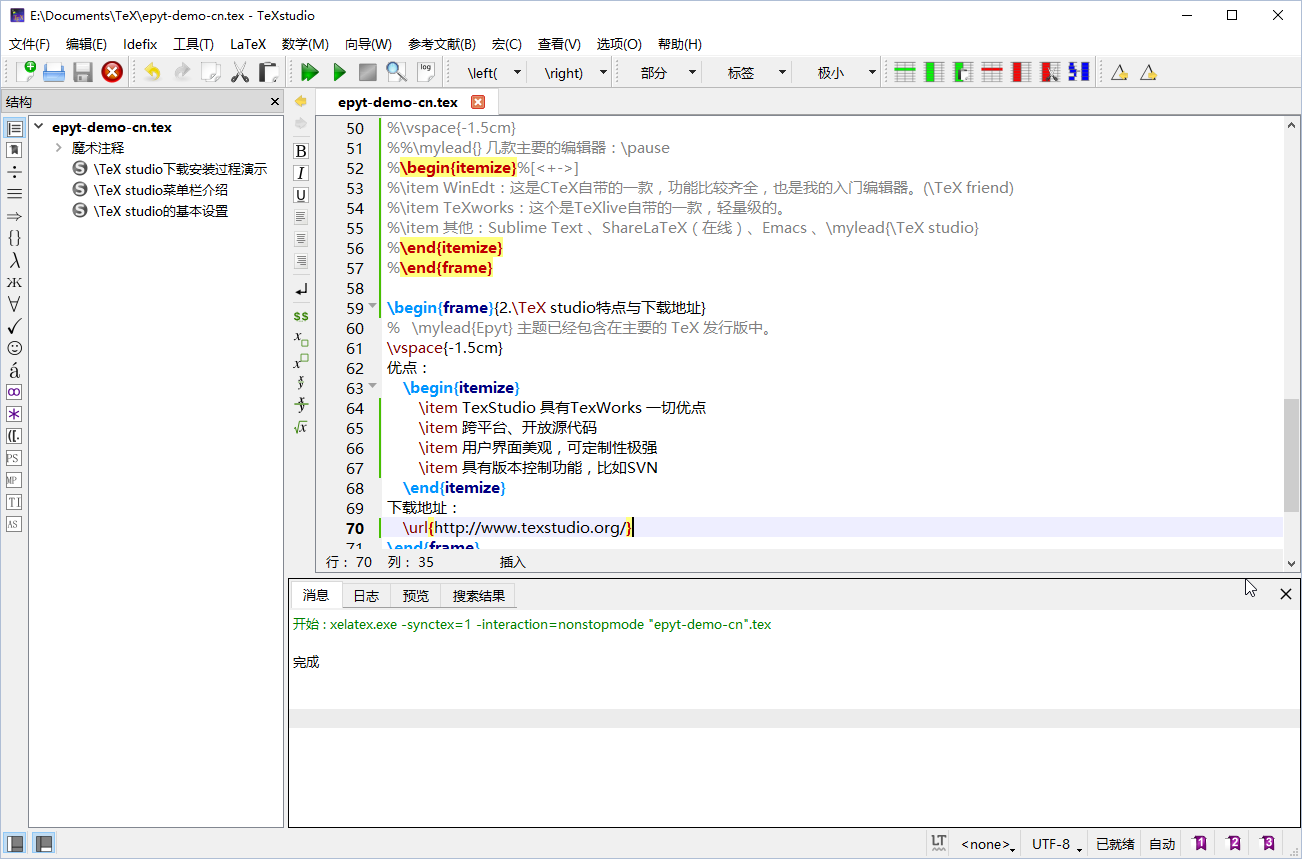
\includegraphics[width=1.00\linewidth]{TeXstudio_Windows}
		\caption{Windows 界面}
		\label{fig:texstudiowindows}
	\end{figure}
	
\end{frame}
\begin{frame}
\begin{figure}
	\centering
	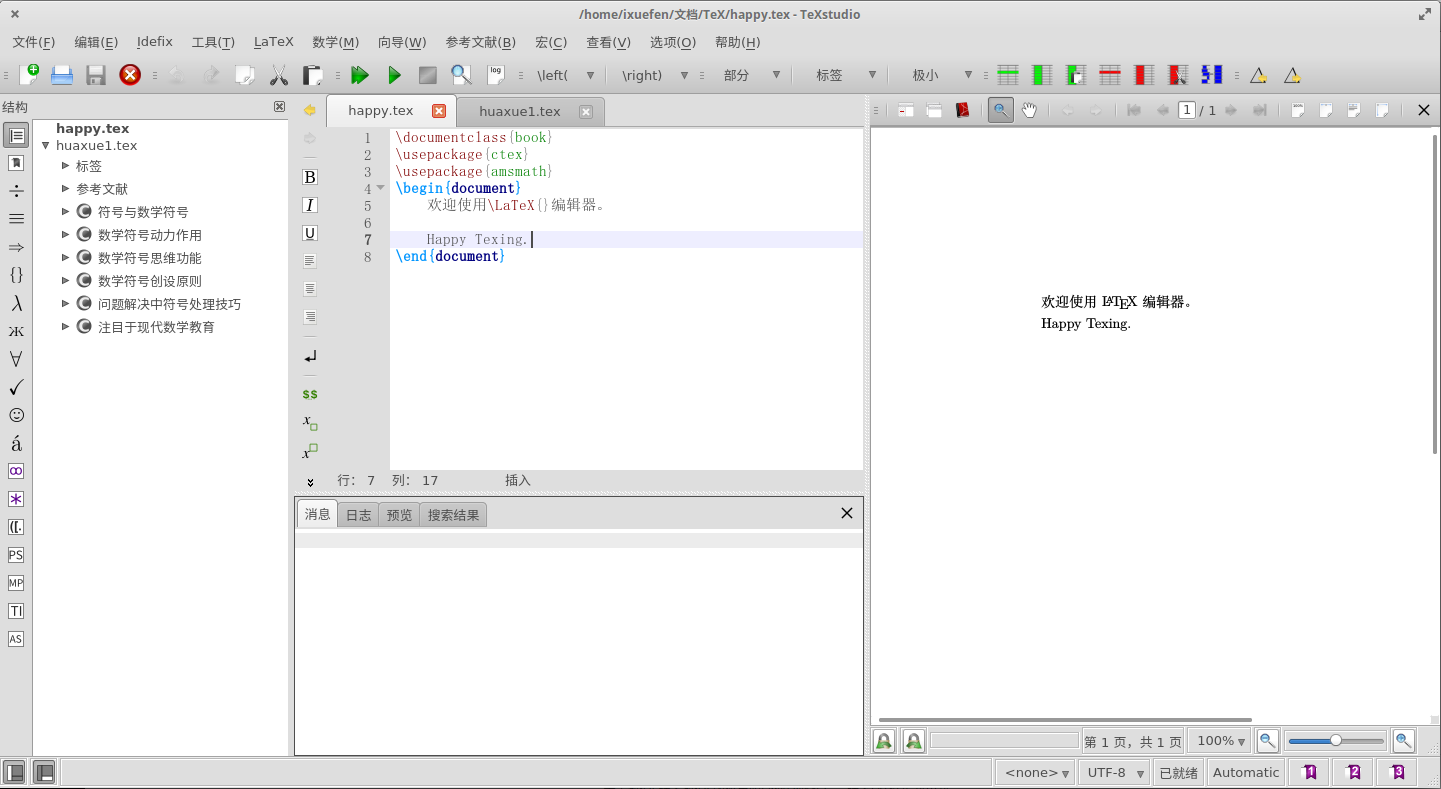
\includegraphics[width=1.0\linewidth]{TeXstudio_linux}
	\caption{Linux 界面}
	\label{fig:texstudiolinux}
\end{figure}
%$\mathrm{sin}x$	
\end{frame}
\begin{frame}
	\frametitle{windows 安装过程}
	\begin{itemize}
		\item 安装TeXLive 2016或 MikTeX,优先推荐安装TeXLive。
		\item 根据系统选择版本,可选安装便携版本。
		\item 推荐先安装TeXlive,后安装TeXstudio。
	\end{itemize}
\end{frame}
\begin{frame}
	注意:本软件更新比较频繁,下载版本号请以实际下载为准
	\begin{figure}
		\centering
		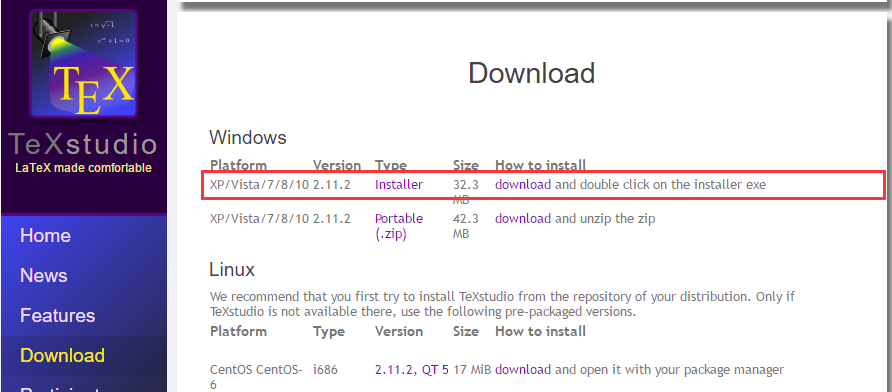
\includegraphics[width=0.7\linewidth]{Windows_install}
		\caption{windows 下载截图}
		\label{fig:windowsinstall}
	\end{figure}
\end{frame}
\begin{frame}
	\frametitle{linux 环境下安装}
	\begin{itemize}
		\item 直接去官方网站下载相对应系统版本软件包,双击安装。
		\item 命令行安装(注意系统环境)。例如 Unbutu 下使用sudo apt isntall texstudio。apt可以替换成yum或dnf。
		\item 源代码安装(不推荐,本软件对各个版本 linux 支持极好,一般不推荐源码安装)
	\end{itemize}
\end{frame}
\section{\TeX studio菜单栏介绍}
\section{\TeX studio的基本设置与使用技巧}
\end{document}

